\documentclass{../../slides-style}

\slidetitle[Часть 1: синтаксический анализ вообще]{Синтаксический анализ}{19.04.2024}

\begin{document}
    
    \begin{frame}[plain]
        \titlepage
    \end{frame}

    \section{Введение}

    \begin{frame}
        \frametitle{Фазы компиляции}
        \begin{center}
            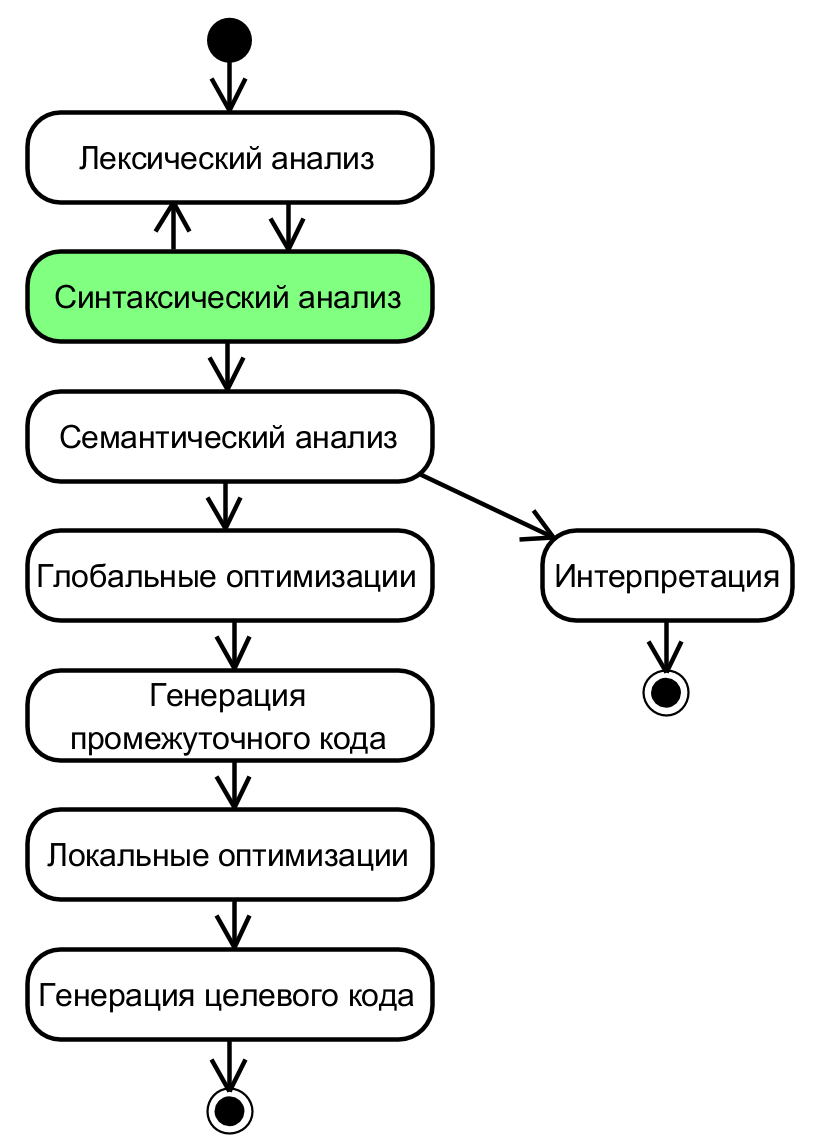
\includegraphics[height=0.8\textheight]{compilerPhases.png}
        \end{center}
    \end{frame}

    \begin{frame}
        \frametitle{Книжка}
        \framesubtitle{Must read}
        \begin{columns}
            \begin{column}{0.6\textwidth}
                А. Ахо, Р. Сети, Дж. Ульман, М. Лам. Компиляторы. Принципы, технологии, инструменты.
                \begin{itemize}
                    \item Так же известна как ``Книга дракона'' (``Dragonbook'')
                \end{itemize}
            \end{column}
            \begin{column}{0.4\textwidth}
                \begin{center}
                    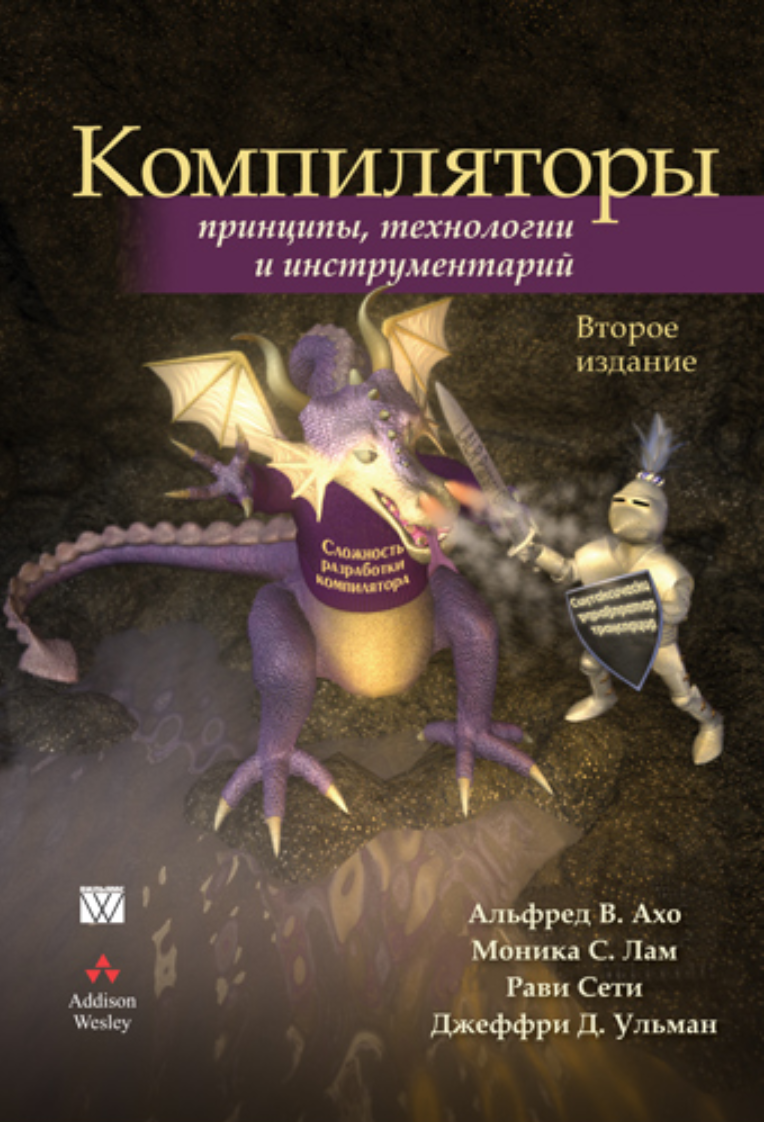
\includegraphics[width=0.7\textwidth]{dragonbook.png}
                \end{center}
            \end{column}
        \end{columns}
    \end{frame}

    \begin{frame}
        \frametitle{Синтаксический анализ}
        \begin{itemize}
            \item Анализ последовательности токенов с целью выяснить синтаксическую структуру
            \begin{itemize}
                \item Сопоставление с формальной грамматикой
            \end{itemize}
            \item Строит структуру данных, представляющую разобранный по синтаксическим правилам документ
            \begin{itemize}
                \item Чаще всего, абстрактное синтаксическое дерево (Abstract Syntax Tree, AST)
                \item Бывает ещё дерево разбора (Parse tree) --- содержит все токены из входной строки, в явном виде обычно не строится
            \end{itemize}
        \end{itemize}
        \begin{center}
            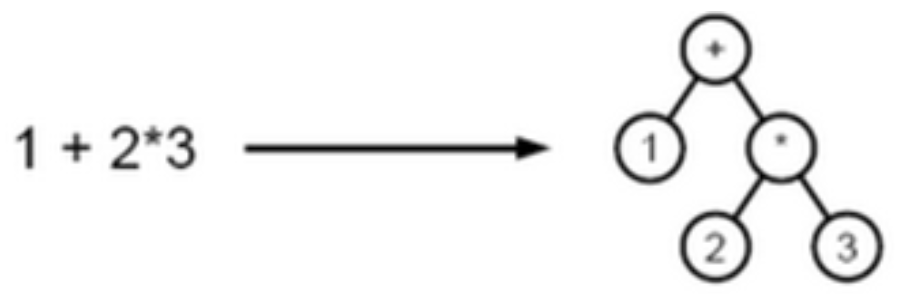
\includegraphics[width=0.4\textwidth]{parsing.png}
        \end{center}
    \end{frame}

    \begin{frame}
        \frametitle{Другие задачи синтаксического анализа}
        \begin{itemize}
            \item Диагностика ошибок
            \item Восстановление после ошибок
            \begin{itemize}
                \item Режим паники
                \item Коррекция
                \item Грамматические правила, обнаруживающие ошибки 
                \begin{itemize}
                    \item ``Предсказание ошибок''
                \end{itemize}
            \end{itemize}
            \item Привязка --- определение для каждой синтаксической конструкции её места в коде
        \end{itemize}
    \end{frame}

    \section{Теория формальных языков}

    \subsection{Формальные грамматики}

    \begin{frame}
        \frametitle{Формальные грамматики}
        \begin{itemize}
            \item Терминал --- символ входной строки для синтаксического анализатора (токен)
            \begin{itemize}
                \item Для лексического анализа входная строка состоит из букв, для синтаксического --- из токенов
            \end{itemize}
            \item Нетерминал --- объект, представляющий сложную синтаксическую конструкцию
            \item Грамматика, формально: $(\Sigma, N, P, S)$, где
            \begin{itemize}
                \item $\Sigma$ --- множество терминалов
                \item $N$ --- множество (алфавит) нетерминальных символов
                \item $P$ --- продукции, функции вида <<цепочка символов>> $\rightarrow$ <<цепочка символов>>, где слева в цепочке есть хотя бы один нетерминал
                \begin{itemize}
                    \item $P: (\Sigma \cup N)^* N\ (\Sigma \cup N)^* \rightarrow (\Sigma \cup N)^*$
                \end{itemize}
                \item $S$ --- стартовый символ, $S \in N$
            \end{itemize}
        \end{itemize}
    \end{frame}

    \begin{frame}[fragile]
        \frametitle{Пример грамматики}
        \begin{minted}{text}
E ::= E + E
      | E - E
      | -E
      | (E)
      | NUMBER

NUMBER ::= 1 | 2 | 3 | ... | 9
        \end{minted}
    \end{frame}

    \subsection{Иерархия Хомского}

    \begin{frame}
        \frametitle{Иерархия Хомского}
        \begin{itemize}
            \item Регулярные языки (языки типа 3) --- задаются регулярными выражениями, разбираются конечными автоматами
            \item Контекстно-свободные грамматики --- грамматики, у которых слева в продукциях может быть только один символ (нетерминал)
            \begin{itemize}
                \item Пример с предыдущего слайда --- КС-грамматика
                \item Разбираются стековыми автоматами (например, рекурсивным спуском)
            \end{itemize}
            \item Контекстно-зависимые грамматики --- в левой части может быть нетерминал и ``контекст'', нетерминал раскрывается в правой части
            \begin{itemize}
                \item Разбираются линейно ограниченными недетерминированными машинами Тьюринга (то есть, всё плохо)
            \end{itemize}
            \item Языки типа 0 --- грамматики без ограничений на вид продукций
            \begin{itemize}
                \item Разбираются машинами Тьюринга (то есть всё очень плохо)
            \end{itemize}
        \end{itemize}
    \end{frame}

    \begin{frame}
        \frametitle{В реальной жизни}
        \begin{itemize}
            \item Регулярные языки --- регэкспы, весь лексический анализ
            \begin{itemize}
                \item Не умеют считать, поэтому грамматики вида $a^nb^n$ (скобочные последовательности) им не под силу
                \item Не могут в иерархические структуры, никогда не парсите регэкспами HTML
            \end{itemize}
            \item Контекстно-свободные грамматики --- грамматики большинства современных языков программирования
            \begin{itemize}
                \item Не могут в анализ типов
            \end{itemize}
            \item Контекстно-зависимые грамматики --- грамматика C++ и некоторых неаккуратных мест в других языках
            \begin{itemize}
                \item Пример: \mintinline{cpp}|A<B> c;| --- либо \mintinline{cpp}|class A<T> {}|, либо \mintinline{cpp}|int A; int B; int c;|
            \end{itemize}
            \item Языки типа 0 --- естественные языки (да, их тоже анализируют грамматиками, и вообще, Хомский был лингвистом)
        \end{itemize}
    \end{frame}

    \subsection{Вывод}

    \begin{frame}
        \frametitle{Вывод в грамматике}
        \begin{itemize}
            \item Формально, если есть грамматика $G = (\Sigma, N, P, S)$, то вывод, $\Rightarrow_G$ --- бинарное отношение на строках
            \begin{itemize}
                \item $x \Rightarrow_G y \iff \exists u, v, p, q \in (\Sigma \cup N)^*: (x = upv) \wedge (p \rightarrow q \in P) \wedge (y = uqv)$
                \item Неформально, шаг вывода --- применение одной из продукций
            \end{itemize}
            \item $\Rightarrow_G^*$ --- рефлексивное транзитивное замыкание $\Rightarrow_G$
            \begin{itemize}
                \item $x \Rightarrow_G^* y$ --- существует конечная последовательность применений продукций грамматики, которая по x делает y
                \item Говорят, <<$y$ выводится из $x$>>
            \end{itemize}
            \item \textit{Порождение} --- последовательность шагов вывода
            \item $L(G)$ --- $\{w \in \Sigma^* | S \Rightarrow_G^* w\}$ --- язык, порождаемый грамматикой $G$
        \end{itemize}
    \end{frame}

    \begin{frame}[fragile]
        \frametitle{Пример}
        Грамматика:
        \begin{minted}{text}
E ::= E + E
      | E * E
      | -E
      | (E)
      | id
        \end{minted}
        
        Входная строка: \mintinline{text}|-(id + id)|
        
        Порождения:
        \begin{itemize}
            \item Левое: \mintinline{text}|E => -E => -(E) => -(E + E) => -(id + E) => -(id + id)|
            \item Правое: \mintinline{text}|E => -E => -(E) => -(E + E) => -(E + id) => -(id + id)|
        \end{itemize}
    \end{frame}

    \subsection{Проблемы грамматик}

    \begin{frame}
        \frametitle{Левая рекурсия}
        \begin{columns}[t]
            \begin{column}{0.5\textwidth}
                Проблема:
                $$A \rightarrow Aa\ |\ b$$
            \end{column}
            \begin{column}{0.5\textwidth}
                Решение: 
                $$A \rightarrow bA'$$
                $$A' \rightarrow aA'\ |\ \epsilon$$
            \end{column}
        \end{columns}
        \begin{columns}[t]
            \begin{column}{0.5\textwidth}
                Пример:
                
                $$E \rightarrow E + T\ |\ T$$
                $$T \rightarrow T * F\ |\ F$$
                $$F \rightarrow (E)\ |\ id$$
            \end{column}
            \begin{column}{0.5\textwidth}
                Пример:

                $$E \rightarrow TE'$$
                $$E' \rightarrow +TE'\ |\ \epsilon$$
                $$T \rightarrow FT'$$
                $$T' \rightarrow *FT'\ |\ \epsilon$$
                $$F \rightarrow (E)\ |\ id$$
            \end{column}
        \end{columns}
    \end{frame}

    \begin{frame}
        \frametitle{Неоднозначность}
        Строка: \mintinline{text}|id + id * id|

        Грамматика (как была): \mintinline{text}!E ::= E + E | E * E | -E | (E) | id!

        Вывод:
        \begin{columns}
            \begin{column}{0.5\textwidth}
                $$E \Rightarrow E + E$$
                $$\Rightarrow id + E$$
                $$\Rightarrow id + E * E$$
                $$\Rightarrow id + id * E$$
                $$\Rightarrow id + id * id$$
                \begin{center}
                    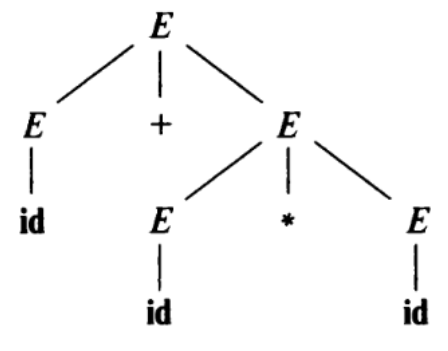
\includegraphics[width=0.5\textwidth]{ambiguousGrammarA.png}
                \end{center}
            \end{column}
            \begin{column}{0.5\textwidth}
                $$E \Rightarrow E * E$$
                $$\Rightarrow E + E * E$$
                $$\Rightarrow id + E * E$$
                $$\Rightarrow id + id * E$$
                $$\Rightarrow id + id * id$$
                \begin{center}
                    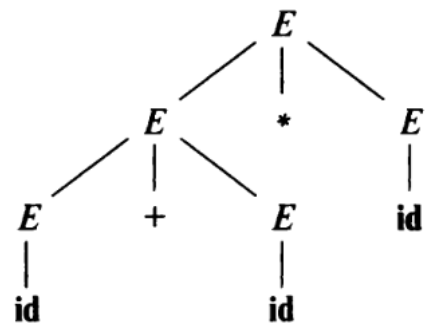
\includegraphics[width=0.5\textwidth]{ambiguousGrammarB.png}
                \end{center}
            \end{column}
        \end{columns}
    \end{frame}

    \subsection{Алгоритмы}

    \begin{frame}
        \frametitle{Алгоритмы разбора}
        \begin{itemize}
            \item Нисходящий разбор --- начинаем со стартового нетерминала, пытаемся построить входную строку
            \begin{itemize}
                \item Рекурсивный спуск
                \item LL-анализ
            \end{itemize}
            \item Восходящий разбор --- пытаемся найти во входной строке последовательность терминалов и нетерминалов и свернуть её в нетерминал
            \begin{itemize}
                \item LR-анализ
            \end{itemize}
        \end{itemize}
    \end{frame}

    \begin{frame}
        \frametitle{Пример}
        \framesubtitle{Нисходящий разбор с построением левого порождения}
        \begin{center}
            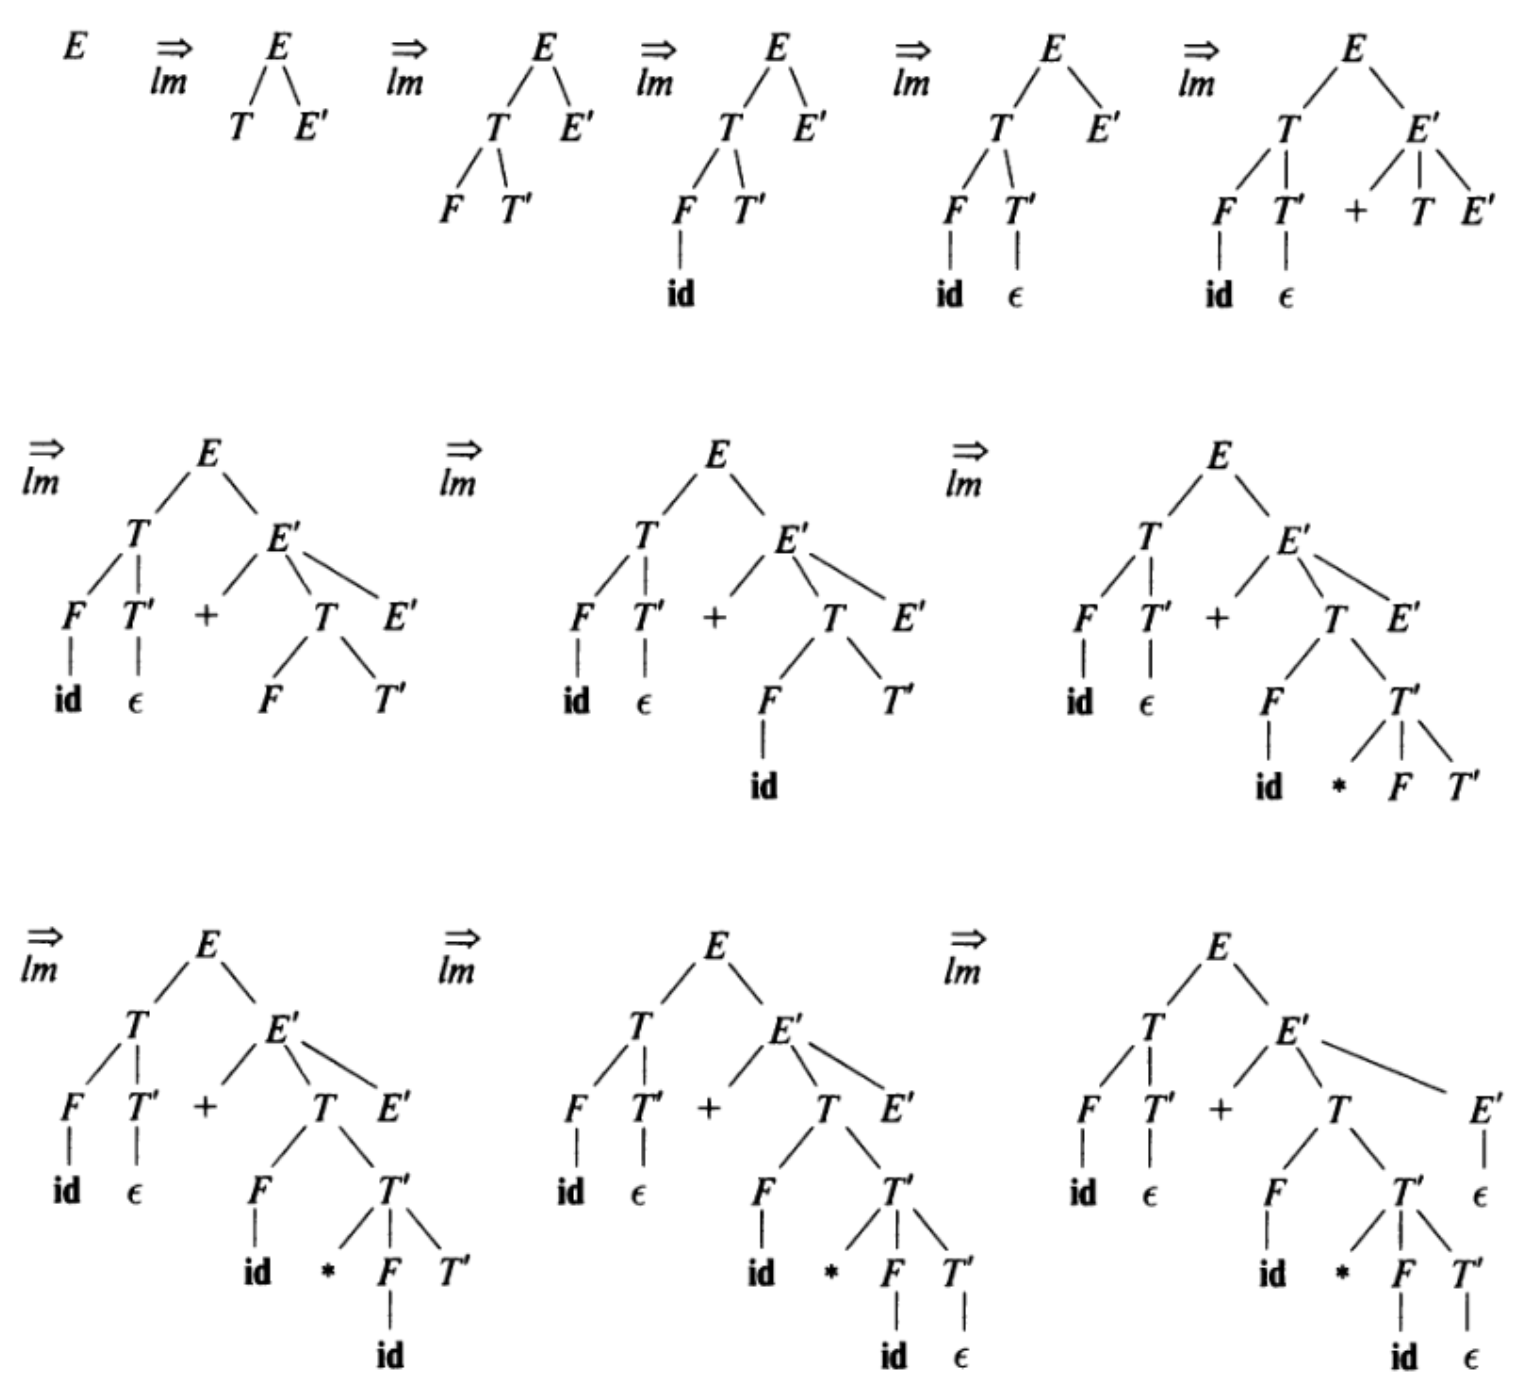
\includegraphics[width=0.65\textwidth]{topDownAnalysis.png}
        \end{center}
    \end{frame}

    \begin{frame}
        \frametitle{FIRST($\alpha$) и FOLLOW($\alpha$)}
        Пусть $\alpha$ --- строка из нетерминалов и терминалов
        \begin{itemize}
            \item FIRST($\alpha$) --- множество всех терминалов, с которых может начинаться $\alpha$
            \begin{itemize}
                \item Считается рекурсивно, раскрытием нетерминальных символов
            \end{itemize}
            \item FOLLOW($\alpha$) --- множество всех терминалов, которые могут стоять за $\alpha$ в выводе в грамматике G
            \begin{itemize}
                \item Считается через FIRST во всех цепочках выводов, в которых может встречаться $\alpha$
                \item $\epsilon$-продукции требуют особого внимания
            \end{itemize}
        \end{itemize}
        Зачем:
        \begin{itemize}
            \item FIRST позволяет выбрать из альтернативных продукций
            \item FOLLOW --- чтобы выбрать между $\epsilon$-продукцией и какой-то другой
        \end{itemize}
    \end{frame}

    \begin{frame}[fragile]
        \frametitle{Рекурсивный спуск}
        \begin{itemize}
            \item По одной функции на нетерминал
            \item Просмотр строки слева направо
        \end{itemize}

        \begin{algorithm}[H]
            Выбираем продукцию $A \rightarrow X_1X_2...X_k$\;
            \For{i от 1 до k}{
                \uIf{$X_i$ -- нетерминал}{
                    Вызов функции $X_i()$\;
                } 
                \uElseIf{$X_i$ равно текущему символу $a$}{
                    Переходим к следующему символу\;
                }
                \Else{
                    Обнаружена ошибка\;
                }
            }
        \end{algorithm}
    \end{frame}

    \subsection{Запись грамматик}

    \begin{frame}
        \frametitle{BNF}
        \framesubtitle{Форма Бэкуса-Наура}
        \begin{itemize}
            \item В угловых скобках --- нетерминал (<literal>)
            \item ::= --- определение (<brackets> ::= '(' | ')')
            \item | --- альтернатива
        \end{itemize}
        Пример: \mintinline{text}/<expr> ::= <term>|<expr><addop><term>/
    \end{frame}

    \begin{frame}[fragile]
        \frametitle{Пример}
        \framesubtitle{BNF, записанная в синтаксисе BNF}
        \begin{footnotesize}
            \begin{minted}{text}
<syntax> ::= <rule> | <rule> <syntax>
<rule> ::= <opt-whitespace> "<" <rule-name> ">" <opt-whitespace> 
        "::=" <opt-whitespace> <expression> <line-end>
<opt-whitespace> ::= " " <opt-whitespace> | ""
<expression> ::= <list> | <list> <opt-whitespace> "|" <opt-whitespace> <expression>
<line-end> ::= <opt-whitespace> <EOL> | <line-end> <line-end>
<list> ::= <term> | <term> <opt-whitespace> <list>
<term> ::= <literal> | "<" <rule-name> ">"
<literal> ::= '"' <text1> '"' | "'" <text2> "'"
<text1> ::= "" | <character1> <text1>
<text2> ::= '' | <character2> <text2>
<character> ::= <letter> | <digit> | <symbol>
<character1> ::= <character> | "'"
<character2> ::= <character> | '"'
<rule-name> ::= <letter> | <rule-name> <rule-char>
<rule-char> ::= <letter> | <digit> | "-"
            \end{minted}
        \end{footnotesize}
    \end{frame}

    \begin{frame}
        \frametitle{Расширенная форма Бэкуса-Наура}
        \begin{itemize}
            \item \{ \} --- 0 или более повторений
            \item {[ ]} --- 0 или 1 раз (опционально)
            \item ( ) --- группировка
            \item , --- конкатенация
            \item Вариантов синтаксиса EBNF больше, чем звёзд на небе
        \end{itemize}
    \end{frame}

    \begin{frame}[fragile]
        \frametitle{Пример}
        \framesubtitle{EBNF, записанная в синтаксисе EBNF}
        \begin{footnotesize}
            \begin{minted}{text}
character = letter | digit | symbol | "_" ;
identifier = letter , { letter | digit | "_" } ;
terminal = "'" , character , { character } , "'" 
         | '"' , character , { character } , '"' ;
lhs = identifier ;
rhs = identifier
     | terminal
     | "[" , rhs , "]"
     | "{" , rhs , "}"
     | "(" , rhs , ")"
     | rhs , "|" , rhs
     | rhs , "," , rhs ;
rule = lhs , "=" , rhs , ";" ;
grammar = { rule } ;
            \end{minted}
        \end{footnotesize}
    \end{frame}

    \section{Синтаксический анализ в ФП}

    \subsection{Парсер-комбинаторы}

    \begin{frame}
        \frametitle{Парсер-комбинаторы}
        \begin{itemize}
            \item Основная идея --- а давайте рассматривать парсер как композицию более простых парсеров
            \begin{itemize}
                \item Определим примитивные парсеры и комбинаторы, строящие парсеры по парсерам
            \end{itemize}
            \item По сути, удобная запись рекурсивного спуска
            \begin{itemize}
                \item Не всегда, иногда используются ``настоящие'' преобразования грамматик
                \begin{itemize}
                    \item Например, Meerkat
                \end{itemize}
            \end{itemize}
            \item Пример --- FParsec
            \begin{itemize}
                \item Порт известной библиотеки Parsec (Haskell)
                \item Рассмотрим \url{http://www.quanttec.com/fparsec/tutorial.html}
            \end{itemize}
        \end{itemize}
    \end{frame}

\end{document}
